\chapter{Introducción específica} % Main chapter title

\label{Chapter2}



%----------------------------------------------------------------------------------------
%	SECTION 1
%----------------------------------------------------------------------------------------
Esta sección presenta una breve introducción técnica a las herramientas hardware y software utilizadas en el trabajo.

\section{Tecnologías de hardware y firmware utilizadas}


\subsection{Robot de exploración ambiental}

Como dispositivo hardware se utilizó el robot de exploración ambiental desarrollado en el marco de la carrera de Especialización de Sistemas Embebidos \citep{cese_gonzalo_memoria}. En la siguiente imagen (\ref{fig:Robot_y_Joystick_1}) se puede apreciar una foto del mismo.


\begin{center}
   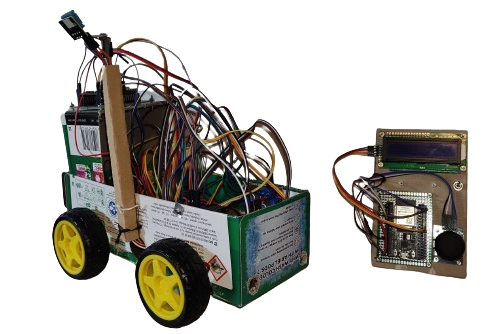
\includegraphics[scale=0.5]{Robot_y_Joystick_1}
   \captionof{figure}{Robot de exploración ambiental.}
   \label{fig:Robot_y_Joystick_1}
\end{center}

El robot de exploración ambiental es un sistema embebido desarrollado sobre \cite{ESP32} utilizando el marco de desarrollo ESP-IDF \cite{ESPIDF_home} de \textit{Espressif Systems} y FreeRTOS (Free Real-Time Operating System) \citep{FreeRTOS} como sistema operativo. Sus principales funciones son la exploración de terrenos de forma controlada por joystick y el la obtención de ciertos parámetros ambientales como luminosidad, presión atmosférica, temperatura y humedad.



\section{Tecnologías backend utilizadas}


\subsection{Amazon Web Services}

AWS (\textit{Amazon Web Services}) \citep{aws}  es una de las principales plataformas de servicios en la nube pública proporcionada por Amazon, que ofrece una amplia gama de productos y herramientas para computación, almacenamiento, bases de datos, redes, inteligencia artificial, seguridad y herramientas de desarrollo.


\subsection{AWS App Runner}

AWS App Runner \citep{aws_app_runner} es un servicio completamente administrado de AWS que permite implementar y ejecutar aplicaciones web y servicios de forma rápida, sin tener que gestionar instancias de infraestructura. Está diseñado para simplificar el proceso de implementación y escalado automático de aplicaciones y permite aplicaciones directamente desde el código fuente o desde contenedores Docker.



\subsection{AWS Glue}

AWS Glue \citep{aws_glue} es un servicio totalmente administrado de AWS diseñado para facilitar la extracción, transformación y carga de datos (ETL) en la nube que permite a los usuarios descubrir, preparar y combinar datos de múltiples fuentes para su análisis y almacenamiento en data lakes, data warehouses o bases de datos. Resulta útil para proyectos de Big Data y análisis de datos ya que brinda un servicio de catálogo de datos, asistencia para la generación de código ETL y un servicio de ejecución de trabajos de procesamiento paralelo.


\subsection{AWS S3}

AWS S3 (\textit{Simple Storage Service}) \citep{aws_s3} es un servicio de almacenamiento de objetos proporcionado por AWS totalmente administrado. Está diseñado para almacenar y recuperar cualquier cantidad de datos desde cualquier lugar, de forma segura, escalable y económica. Es ideal para almacenamiento de datos no estructurado de grandes volúmenes, sitios web estáticos, archivos multimedia, copias de seguridad, etc.

\subsection{AWS Athena}

AWS Athena \citep{aws_athena} es un servicio de análisis de datos serverless proporcionado por AWS que permite consultar directamente datos almacenados en Amazon S3 y los esquemas definidos en Glue, utilizando SQL estándar sin necesidad de configurar ni administrar servidores. Es ideal para analizar grandes volúmenes de datos de forma rápida y económica.



\subsection{MQTT}

MQTT (\textit{Message Queuing Telemetry Transport}) \citep{mqtt_spec} es un protocolo de comunicación asincrónico, ligero y orientado a mensajes, diseñado específicamente para dispositivos con recursos limitados y redes de baja ancho de banda. Es ampliamente utilizado en casos de uso IoT para la transmisión de datos en tiempo real entre dispositivos, sensores y aplicaciones. Utiliza un modelo de comunicacion basado en publish/subscribe y una estructura de datos basada en topics a los cuales los componentes clientes se conectan a un servicio broker para publicar o recibir notificaciones. 

\subsection{AWS IoT Core}

AWS IoT Core \citep{aws_iot_core} es un servicio totalmente administrado de AWS que permite conectar dispositivos IoT (Internet of Things) a la nube de manera segura y confiable. Proporciona una infraestructura escalable para recopilar, procesar y analizar datos de dispositivos en tiempo real, así como para interactuar con otros servicios de AWS a los que se redirigen los mensajes recibidos mediante la configuración de reglas. Tiene soporte para varios protocolos de comunicaciones, entre los que se destacan principalmente MQTT, HTTP/S, WebSockets y LoRaWAN.

\subsection{Node.js}

Node.js \citep{nodejs} es un entorno de ejecución de código abierto, construido sobre el motor de JavaScript V8 de Google Chrome. Aunque debido a su diseño puede ser utilizado para desarrollar aplicaciones backend de propósito general que requieran escalabilidad y rendimiento, es utilizado principalmente como servidor web. Para su funcionamiento utiliza un modelo single-thread de event loop con I/O no bloqueante, por lo que gestiona un bucle de eventos encolados y los procesa invocando sus callbacks de forma asincrónica sin realizar bloqueo de entradas y salidas en los puertos de comunicaciones, permitiendo atención de multiples solicitudes y paralelismo de tareas.

\section{Tecnologías Blockchain utilizadas}


\subsection{Ecosistema Ethereum}

Ethereum \citep{ethereum} es una red blockchain pública diseñada para el procesamiento de transacciones de forma descentralizada con almacenamiento distribuido, inmutable y de acceso libre ( \textit{permissionless}). La red se encuentra formada por los nodos de procesamiento, tambien denominados validadores, que tienen como función procesar transacciones y como otras redes blockchain, utiliza una estructura de datos basada en una cadena de bloques, en los cuales se van agrupando las transacciones validadas. 

Ethereum tiene como \textit{token} el Ether cuyo símbolo es ETH y tiene varios usos, pudiendo ser utilizado como criptomoneda de cambio y ahorro entre los usuarios finales de la red, pero también para pagar el gas (costo de ejecución de transacciones y smart contracts) y los fees a los validadores.

El proceso de validación de transacciones y generación de bloques, a partir de la versión 2.0 de Ethereum, utiliza el protocolo PoS (Proof-of-Stake) \citep{PoS} y opera en ranuras de tiempo llamadas slots, con un bloque propuesto aproximadamente cada 12 segundos. 

El primer paso de este proceso es la recolección de transacciones enviadas por los usuarios a la red (por ejemplo, para transferir dinero o ejecutar contratos) y su almacenamiento en un \textit{mempool} temporal. Luego, un validador es seleccionado de forma aleatoria para proponer el siguiente bloque, seleccionando del \textit{mempool} aquellas transacciones con tarifas de gas mas altas para maximizar su recompensa. El validador seleccionado incluye: las transacciones válidas, estado actualizado del sistema, hash del bloque anterior y los datos adicionales como la firma del bloque. Como resultado, este bloque es propuesto al resto de la red, en la que posteriormente, un comité de validadores, seleccionado de forma aleatoria, revisa el bloque verificando que las transacciones sean válidas, el bloque no esté duplicado o malicioso y sea coherente con el estado de la blockchain. Si el bloque es válido, los validadores emiten un voto (attestation) que confirma su aprobación. Si más de 2/3 de los validadores en el comité atestiguan el bloque, se considera finalizado y el bloque es agregado a la cadena de bloques de forma permanente.

El proceso de compensación y penalización de PoS retribuye a los validadores por diferentes acciones, con el fin de mantener la seguridadm, integridad y consenso de la red, aplica una técnica llamada slashing para la penalización por acciones malisiosas o incorrectas durante el procesamiento. El validador que propone el bloque recibe recompensas por bloque y tarifas de gas. Los validadores que votan correctamente para validar bloques también reciben recompensas proporcionales a su participación. Si el validador no presenta comportamiento malicioso o inactividad, no es penalizado. Sin embargo, los validadores pueden perder parte o todo su capital en stak si proponen múltiples bloques en un mismo slot, o votan de manera inconsistente (por ejemplo, intentando atacar la red), o están inactivos durante largos períodos de tiempo.

Antes de la versión 2.0 de Ethereum, se utilizaba otro protocolo de consenso llamado PoW (Proof-of-Work) \citep{PoW}, en el cual los nodos validadores desempeñaban el rol de mineros que competían por la generación del bloque, recompensando al que lo lograba generar y desaprovechando los recursos de cómputo utilizados por los que no lo lograron. El protocolo PoS en la version actual de Ethereum tiene varias ventajas con respecto a PoW consumiendo un 99,9 \% de energía, aumenta la escalabilidad con técnicas de sharding, y reduce las barreras de entrada al no requerir disponer de un hardware costoso para poder participar del proceso de validación.

% *intro a la evm*

Ethereum se diferencia de otras blockchains, como Bitcoin, porque no es solo un libro mayor digital, sino también una plataforma programable en la cual utilizando un SDK se pueden contruir programas denominados \textit{Smart Contracts} que se despliegan y ejecutan en la red. Como se mencionó anteriormente, los Smart Contracts (o contratos inteligentes) son programas informáticos autónomos que se ejecutan en redes blockchain como Ethereum, Solana o Binance Smart Chain. y están diseñados para automatizar, verificar y hacer cumplir acuerdos sin necesidad de intermediarios. Funcionan bajo el principio de si sucede una condición, entonces ejecutar una acción, aunque también pueden ser invocados de forma directa para operaciones de lectura y escritura. Una vez desplegados en la blockchain, no se pueden modificar, y todas las transacciones quedan registradas públicamente. 

El ciclo de vida de los \textit{smart contracts} comienza con su desarrollo utilizando alguno de los lenguajes de programación y SDK disponibles, como por ejemplo Solidity y Truffle. Una vez desarrollado, tras el proceso de compilación se obtiene un ABI \citep{abi} o especificación del contrato en formato JSON que no es enviado a la blockchain, sino que tiene como proposito poder ser utilizado posteriormente para acceder a los atributos y métodos del mismo a la hora de invocarlo. Posteriormente, durante el proceso de despliegue, se genera un binario del contrato que es enviado a la blockchain y tras ser procesado como una transacción mas, queda disponible en la red de manera inmutable. Al estar desplegado y disponible puede ser invocado o ejecutado automaticamente cuando se cumplen ciertas condiciones, generando nuevas transacciónes inmutables procesadas por la red y disponibles para ser consultadas.

Como se mencionó anteriormente, para la invocación a los \textit{smart contracts} se utilizan las dApps como componente de abstracción. Las dApps son aplicaciones que se ejecutan fuera de la blockchain (pudiendo ser por ejemplo un \textit{backend} en Node.js o un \textit{frontend} Javascript) e interactúan con la blockchain a través de ciertas bibliotecas, como por ejemplo, Web3.js \citep{web3}. Para poder acceder a la red, y posteriormente invocar el \textit{smart contract}, la dApp necesita utilizar un endpoint RPC publicado por cualquier nodo de la red y disponer de la especificación ABI del \textit{smart contract} obtenido durante su compilación (y no se disponible en la red).

Ethereum consta de varias redes disponibles para distintos propósitos. La Mainnet \citep{mainnet} es su red principal para usos productivos. Además existen múltiples \textit{testnets}, o redes de prueba, como Sepolia \citep{sepolia} y Holesky \citep{holesky} entre otras, disponibles para ser usadas durante el desarrollo y evaluación de soluciones blockchain en entornos productivos sin necesidad de pagar con fondos reales. Cada red tiene sus propias características y configuración de parámetros como el consenso, gas \textit{fees} y emisión de bloques.


\subsection{Solidity}

Solidity \cite{solidity} es un lenguaje de programación de alto nivel, orientado a contratos inteligentes, específicamente diseñado para funcionar en la Ethereum Virtual Machine (EVM). Fue creado en 2014 por Gavin Wood, Christian Reitwiessner y otros desarrolladores de Ethereum. Su sintaxis es similar a JavaScript, Python y C++, lo que facilita el aprendizaje para desarrolladores familiarizados con esos lenguajes. 


\subsection{Biblioteca Web3.js}

web3.js \citep{web3} es una biblioteca de JavaScript que permite interactuar con la blockchain de Ethereum y otros protocolos compatibles con Ethereum Virtual Machine (EVM). Proporciona una forma sencilla de conectarse a nodos de Ethereum, realizar transacciones y leer datos de contratos inteligentes, directamente desde aplicaciones web o Node.js.


\subsection{Ganache}

Ganache \cite{ganache_website} es una herramienta de desarrollo de Ethereum que permite crear una blockchain local para probar, desarrollar y depurar contratos inteligentes y dApps de forma rápida y segura. Es parte del conjunto de herramientas de Truffle Suite y es ampliamente utilizada por desarrolladores para simular una red Ethereum sin necesidad de usar una red pública como Mainnet o Testnets (Goerli, Sepolia).


\subsection{Truffle}

Truffle \cite{truffle_website} es un framework de desarrollo para Ethereum y otras blockchains compatibles con EVM (Ethereum Virtual Machine). Es parte de Truffle Suite y proporciona herramientas para compilar, desplegar y probar contratos inteligentes, además de facilitar la gestión de proyectos basados en Web3. Truffle automatiza gran parte del proceso de desarrollo de dApps, reduciendo errores y mejorando la eficiencia.

\subsection{Alchemy}

Como se mencionó mas arriba, la dApp, implementada como un servicio Node.js, es la responsable de invocar al Smart Contract desplegado en Ethereum utilizando un endpoint RPC publicado por cualquier nodo de la red. Debido a que los nodos públicos de la red pueden resultar limitados por motivos de seguridad, rendimiento y confiabilidad, resulta una mejor alternativa levantar un nodo EVM administrado o consumir esto como un servicio de un proveedor como Alchemy. Alchemy \cite{alchemy_website} es una plataforma de desarrollo blockchain que proporciona herramientas e infraestructura para crear y gestionar dApps en Ethereum y otras redes compatibles con EVM. Es conocida como el "AWS de Blockchain" debido a que ofrece nodos como servicio y herramientas para facilitar la interacción con la blockchain sin necesidad de que los desarrolladores configuren y mantengan sus propios nodos. En el trabajo actual, se utilizó Alchemy como punto de integración entre la dApp y los Smart Contracts.

\subsection{Etherscan}

Etherscan \cite{etherscan} es un explorador de bloques y plataforma de análisis para la red Ethereum. Permite a los usuarios buscar, verificar y rastrear transacciones, contratos inteligentes, direcciones de billeteras y otros datos en tiempo real. Es una herramienta fundamental para los desarrolladores y usuarios de Web3, ya que ofrece transparencia y acceso abierto a la información almacenada en la blockchain de Ethereum, tanto la Mainnet como las redes de prueba (Sepolia, Holesky, etc).

\subsection{Metamask}

MetaMask \cite{metamask} es una billetera digital y extensión de navegador (también disponible como aplicación móvil) que permite a los usuarios interactuar con blockchains basadas en Ethereum y otros ecosistemas compatibles con Ethereum, como Binance Smart Chain (BSC) y Polygon. Es una herramienta fundamental para interactuar con aplicaciones descentralizadas (dApps), contratos inteligentes y realizar transacciones de criptomonedas directamente desde tu navegador.
En el presente trabajo se utilizó para almacenar los fondos en ETH obtenidos a través de faucets necesarios para pagar el gas de las transacciones.

\section{Tecnologías de desarrollo utilizadas}


%\begin{center}
%\end{center}
%\includegraphics[scale=0.25]{espressif}

% \footnotetext{Imagen tomada de \cite{espressif-website-esp-idf}}

\subsection{Plataforma Docker}

Docker \cite{docker_website} es un proyecto de código abierto que automatiza el despliegue de aplicaciones dentro de contenedores de software, proporcionando una capa adicional de abstracción y automatización de virtualización de aplicaciones en múltiples sistemas operativos. Docker utiliza características de aislamiento de recursos del kernel Linux, tales como cgroups y espacios de nombres (namespaces) para permitir que contenedores livianos independientes se ejecuten en paralelo de manera aislada evitando la sobrecarga de iniciar y mantener máquinas virtuales.

%\includegraphics[scale=0.15]{docker}



\subsection{Plataforma de CI/CD}
Durante el proceso de desarrollo del producto se utilizó CI/CD (\textit{continuous integration / continuous delivery}) mediante la integración de las siguientes herramientas:

\begin{itemize}
	\item Github \cite{SoftwareTool_Github}: servicio de repositorio y control de versiones de código fuente.
	\item AWS CodePipeline \cite{SoftwareTool_codePipeline}: servicio de compilación, empaquetado y ejecución \textit{builds}.
	\item AWS Elastic Container Registry \cite{SoftwareTool_ECR}: servicio de repositorio y control de versiones de imágenes Docker.
\end{itemize}

El objetivo de esta configuración de servicios es permitir que por cada cambio en el código fuente versionado en el controlador de versiones Github, se dispare un proceso de compilación y ejecución de tests unitarios notificando en tiempo real si dicho cambio agrega o no una falla al actual estado del desarrollo. En caso de pasar satisfactoriamente la compilación y ejecución de los tests entonces se genera una nueva imagen Docker con la última versión del codigo compilado y se versiona en Artifact Registry.

\subsection{Visual Studio Code}

Visual Studio Code \cite{vscode_website} es un editor de código fuente desarrollado por Microsoft para Windows, Linux, macOS y Web. Incluye soporte para la depuración, control integrado de Git, resaltado de sintaxis, finalización inteligente de código, fragmentos y refactorización de código.

%\includegraphics[scale=0.15]{vscode}

\subsection{Sistema operativo Ubuntu}
Ubuntu \cite{ubuntu_website} es una distribución Linux basada en Debian GNU/Linux y patrocinado por Canonical, que incluye principalmente software libre y de código abierto. Puede utilizarse en ordenadores y servidores, está orientado al usuario promedio, con un fuerte enfoque en la facilidad de uso y en mejorar la experiencia del usuario.

%\includegraphics[scale=0.25]{ubuntu}



